\documentclass[a4paper,twoside]{book}
 
\usepackage[english]{babel}
\usepackage[utf8]{inputenc}
%~ \usepackage[dvips]{epsfig} % This package is evil! EVIL I TELL YOU!
\usepackage{a4}
\usepackage{fancyhdr}
\usepackage[official]{eurosym}
 
%Added
\usepackage{amssymb,amsmath}
\usepackage{gensymb}
\usepackage{titlesec}
\usepackage{color, graphicx, caption}
\usepackage{wrapfig}
\usepackage[export]{adjustbox}
\usepackage{subcaption}
\usepackage[nottoc,numbib]{tocbibind}
\usepackage[T1]{fontenc}
\usepackage{microtype}
\usepackage[toc,page]{appendix} 

%%%%% FABIO FA BRUTTE COSE
\newcommand{\includeDir}{include}
\newcommand{\import}[1]{\input{\includeDir/#1}}

% \nobreakhline : \hline that doesn't break pages
\makeatletter
\def\nobreakhline{%
  \noalign{\ifnum0=`}\fi
    \penalty\@M
    \futurelet\@let@token\LT@@nobreakhline}
\def\LT@@nobreakhline{%
  \ifx\@let@token\hline
    \global\let\@gtempa\@gobble
    \gdef\LT@sep{\penalty\@M\vskip\doublerulesep}
  \else
    \global\let\@gtempa\@empty
    \gdef\LT@sep{\penalty\@M\vskip-\arrayrulewidth}
  \fi
  \ifnum0=`{\fi}%
  \multispan\LT@cols
     \unskip\leaders\hrule\@height\arrayrulewidth\hfill\cr
  \noalign{\LT@sep}%
  \multispan\LT@cols
     \unskip\leaders\hrule\@height\arrayrulewidth\hfill\cr
  \noalign{\penalty\@M}%
  \@gtempa}
\makeatother

% \tablesection{# columns}{text} : used to divide thematic groups in a table
\newcommand{\tablesection}[2]{%
  \multicolumn{#1}{c}%
  {%
    #2%
  }%
  \\* \nobreakhline%
}

\newcommand{\code}[1]{\texttt{#1}}
\newcommand{\variable}[1]{\texttt{\textit{#1}}}
\newcommand{\cmdline}[1]{\texttt{#1}}

\newcommand{\addcaption}[2]{%
  \multicolumn{#1}{c}{%
    \textbf{[\autoref*{#2}]}%
  }%
}

% ScheMo deserves a command
\newcommand{\ScheMo}{ScheMo}
\newcommand{\ScheMoTeX}{%
\raise .5ex\hbox {S}%
\kern -.2em\lower .5ex\hbox {\textsc{che}}%
\kern -.12em\raise .1ex\hbox {M}%
\kern -.125em\lower .5ex\hbox {\small O}%
\kern -.125em\TeX{}%
}

\import{fabiopkg}
%%%%% FABIO SMETTE

\titleformat{\chapter}[block]
  {\normalfont\huge\bfseries}{\thechapter.}{1em}{\Huge}
\titlespacing*{\chapter}{0pt}{-19pt}{0pt}
 

\let\cleardoublepage\clearpage
 
\begin{document}

\thispagestyle{empty} \cleardoublepage
\begin{center}
 \LARGE{\textbf{POLITECNICO DI MILANO}}\\
 \mbox{\large{SCHOOL OF INDUSTRIAL AND INFORMATION ENGINEERING}}\\
 \mbox{\Large{\textsc{Biomedical Engineering}} }
\end{center}
\addvspace{1cm}
\begin{figure}[h]
 \centering
 
\includegraphics[width=6cm]{img/polilogo.eps}
\end{figure}
 
\addvspace{1cm}
 
\begin{center}
 \begin{large}
  \textbf{\textsc{Design and realization of a table-top robotic game for motor impaired children}}
 \end{large}
\end{center}
 
\addvspace{3cm}
\begin{Large}
  \begin{tabbing}
     Advisor: \hspace{4pt}  \= Prof. Andrea Bonarini\\
     \\
     \\
     Bachelor Thesis by:
  \end{tabbing}
   
 \begin{tabular}{ l c r }
  Fabio Paini & Beatrice Pazzucconi & Damiano Quadraro \\
  ID 806874 & ID 809830 & ID 806809 \\
 \end{tabular}
 
     \vfill
  \begin{center}
    Academic Year 2015 - 2016
  \end{center}
 
\end{Large}
\newpage


\pagenumbering{Roman}

\tableofcontents
\newpage

\pagenumbering{arabic}

\chapter{Abstract}
Since 1950's playing has been regarded as crucial to proper child's social, personal and physical development. This applies not only to games specifically designed to educate, but also to all forms of playing, that is: \textquotedblleft play for the sake of play\textquotedblright.

Children with disabilities in particular seem to react in an extremely positive way, although they're often secluded from normal children's activities, and therefore are deprived of a valuable opportunity to develop and overcome some of their limitations.

Our work focused on creating a game environment for children with motor impairments and a table-top interface to play it. The game provides kid-friendly interactions and the possibility to play with another child (whether disabled or not), trying to even the participants abilities.

In this relation we explain the various steps taken to design shape and interaction of the game, prototype construction, in prevision of an eventual trial with patients.
Although it may sound obvious, we would like to point out that both the design and construction were entirely carried out by ourselves and almost exclusively with our own means. Therefore, also owing to the little time or poor resources available, we sometimes resolved to solutions different from what we initially planned. This relation separates the design process from realisation, so that it is easy to understand where we had to come to a compromise or alternative solution. Also, options are compared in a future development-perspective, for whoever might like to improve our results.


\chapter{Sommario}
A partire da circa la met\`{a} del secolo scorso, si \`{e} cominciato a prestare un crescente interesse nei confronti della psicologia dei bambini. Ne \`{e} emerso che il gioco rappresenta una parte fondamentale per lo sviluppo corretto del bambino, sotto molteplici punti di vista: fisico, psicologico e sociale. Un aspetto importante di questa scoperta \`{e} inoltre che il gioco non necessita di avere uno scopo prettamente educativo per sortire il suo effetto positivo, ma pu\`{o} anche essere fino a se stesso.

I bambini con disabilit\`{a} beneficiano pi\`{u} degli altri di questi effetti, ma paradossalmente, vengono esclusi da questa possibilit\`{a} spesso, perdendo cos\`{i} l'opportunit\`{a} di superare le loro difficolt\`{a}.

Il nostro progetto si propone di creare un sistema di gioco da tavolo ed un'interfaccia di gioco robotica per bambini affetti da disabilit\`{a} motorie. Il gioco promuove una comunicazione costruttiva nei confronti dell'utente e fornisce l'opportunit\`{a} di avere un secondo giocatore (normodotato o meno), cercando al contempo di portare i due giocatori allo stesso livello.

In questa relazione illustriamo i diversi passaggi effettuati per progettare la forma e l'interfaccia del gioco, la costruzione di un prototipo, in vista di un eventuale test con pazienti.
 
\chapter{Introduction}

By now there is strong evidence in literacy that play is not only a purely leisure activity, but that is fundamental to allow children develop properly. Proof of it is the decision of the U.N.O.\footnote{United Nations Organization} to make play a right of every child. 
\\
Playing:
\begin{itemize}
\item develops social, physical, cognitive, abilities;
\item  improves psychological and emotional strength.
\end{itemize}
What is even more interesting is that it is not necessary for the game to have a specific educational target, but also playing for its own sake serves the purpose. Moreover, there is evidence that  deprivation of playing may affect negatively the child in the future.
\\
Despite this, many children are still denied this opportunity, and this can be due to:
\begin{itemize}
\item living conditions (poverty, wars, exploitation \textellipsis);
\item progressive emphasis on academics in schools and highly scheduled lifestyle trends in middle and upper class families \cite{art4};
\item children disabilities.
\end{itemize}
Consequences of this in adulthood and adolescence may be: (only relating to the second and third classes)
\begin{itemize}
\item  anxiety, depression and lack of self-confidence and self-esteem in general \cite{art4};
\item lowered motivation, dependence on others, underdeveloped social skills with particular regards to disabled children \cite{art9}.
\end{itemize}
Children affected by disabilities seem more prone than the others to suffer the consequences of deprivation of play and proper stimuli. We can define a  \textquotedblleft physical\textquotedblright deprivation (lack of sensory and motor information received by the child), and a \textquotedblleft
 social\textquotedblright deprivation (secondary disabilities as an indirect result of the former). The reasons for this are various, such as physical limitations of the child him/herself, environmental barriers, and social barriers (integration with peers) \cite{art2},\cite{art4},\cite{art8},\cite{art9}.

Recently, many efforts have been made to use technology to assist disabled children. Also a 4-year action supported by the C.O.S.T.\footnote{European Cooperation in Science and Technology} started in 2014 to connect experts and professionals all over Europe (from 28 countries) and spread concern, to ensure children with disabilities are granted their righteous playing. (LUDI \textemdash Play for Children with Disabilities \footnote{\textit\underline{http://www.cost.eu/COST\_Actions/TDP/Actions/TD1309}; \textit\underline{http://www.ludi-network.eu}}) \cite{art3}.

\section{Social Robotics}
Robotics seem particularly promising in this case and have been already employed quite successfully in biomedical environment. In particular it is Social Robotics' aim to develop a natural and productive human-machine interface to improve the quality of playing.
 
\begin{figure}[h]
  \centering
  \begin{subfigure}[b]{0.3\textwidth}
    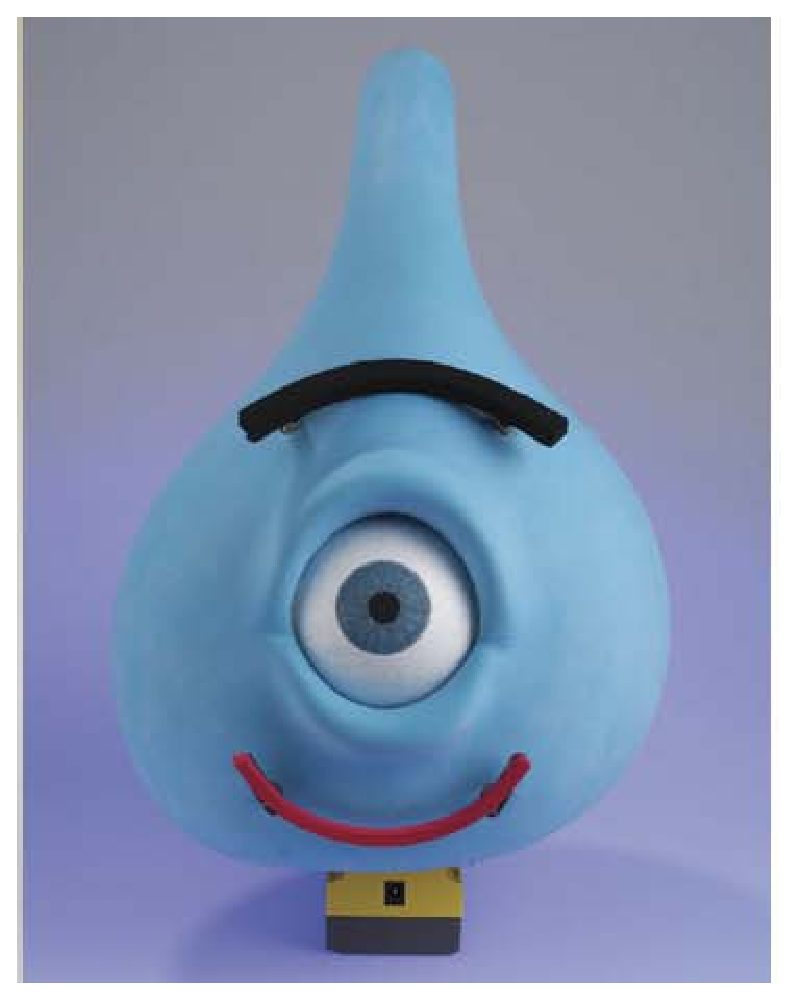
\includegraphics[width=1\linewidth]{img/Bartneck} 
  \end{subfigure}%
  \quad%
  \begin{subfigure}[b]{0.3\textwidth}
    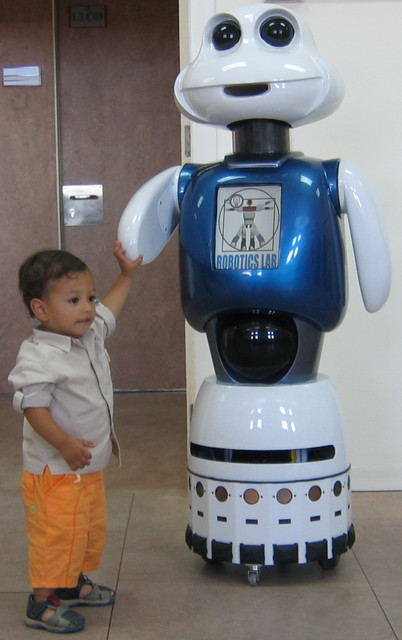
\includegraphics[width=1\linewidth]{img/Salichs}
  \end{subfigure}%
  \quad%
  \begin{subfigure}[b]{0.3\textwidth}
    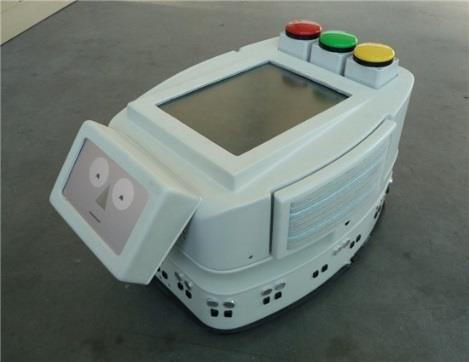
\includegraphics[width=1\linewidth]{img/Heuvel}
  \end{subfigure}
  \begin{subfigure}[t]{0.3\textwidth}
    \caption{Emuu: Bartneck, C., Reichenbach, J., and Breemen, A., 2004}
  \end{subfigure}%
  \quad%
  \begin{subfigure}[t]{0.3\textwidth}
    \caption{Maggie: Miguel A. Salichs, et al., 2006}
  \end{subfigure}%
  \quad%  
  \begin{subfigure}[t]{0.3\textwidth}
    \caption{Van den Heuvel R. et al., 2015}
  \end{subfigure}
  \caption{Examples of Social Robots.}
\end{figure}

Some encouraging experiments have already been carried out in favour of child-robot interface rather than a bare interaction with a tablet or device (for example to measure children's ability to develop language).

In fact, children generally react to the robot with more ease as with an adult, for it doesn't look as inquiring or expectant, as long as the robot is fitted with an opportune appearance (that is, it needs to be dressed up to look child\textendash friendly). Therefore children react more enthusiastically to them as they would with simply a tablet \cite{art12},\cite{art13}.

\section{Related Studies}

Social Robotics potential has been evidenced also in experiments/studies involving disabled children. Patients were mainly children affected by ASD\footnote{Autistic Spectrum Disorders}, motor and generally cognitive disabilities \cite{art1},\cite{art6},\cite{art7},\cite{art10}, or even diabetes \cite{art5}, and much more is still in progress \cite{art11}.

\begin{figure}[h]
 
\begin{subfigure}{6cm}
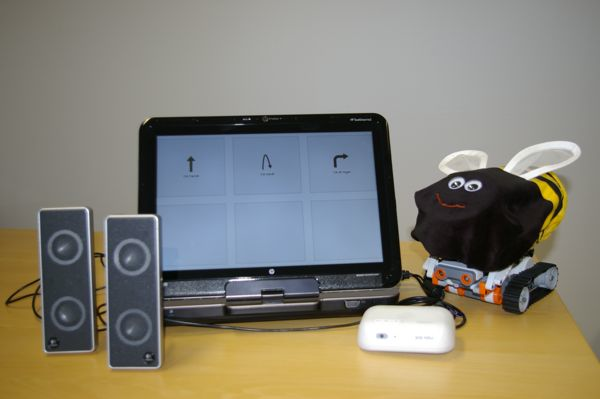
\includegraphics[width=6cm]{img/Ljunglof} 
\captionsetup{width=5cm}
\caption{LEKBOT: Ljungl\"of P. et al., 2011}
\end{subfigure}
\begin{subfigure}{6cm}
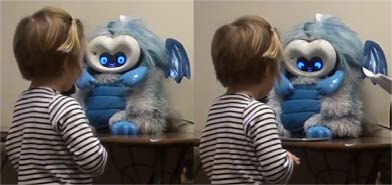
\includegraphics[width=6cm]{img/Westlund}
\captionsetup{width=5cm}
\caption{Westlund J. et al., 2015}
\end{subfigure}

\caption{Examples of social robots used with disabled children(1).}
\end{figure}
Difficulties encountered by researchers were mainly:
\begin{enumerate}
\item low playfulness of patients (whether due to physical impairments or to the child's mood);
\item wide range of possible impairments; that is, every patient, especially those affected by ASD or motor disabilities, has his/her own peculiar situation.
\end{enumerate}
The main limitations of the above\textendash mentioned studies (and in general, studies related to the use of social robotics in children playing) were:

\begin{enumerate}
\item almost exclusive focus over children with ASD, neglecting other disabilities;
\item excessive focus on the educational purpose of the game;
\item lack of possibility to play with other children and therefore improve social skills;
\item excessively complex/simplified game schemes and rules so that the game may be regarded as too hard/boring;
\item excessive/too apparent facilitation of disabled child that undermines challenge.
\end{enumerate}

\begin{figure}[b]

\begin{subfigure}{4.5cm}

\includegraphics[width=4cm, height=3cm]{img/Cabibihan}
\captionsetup{width=4cm}
\caption{Charlie: J. Cabibihan et al., 2013}
\end{subfigure}
\begin{subfigure}{4cm}
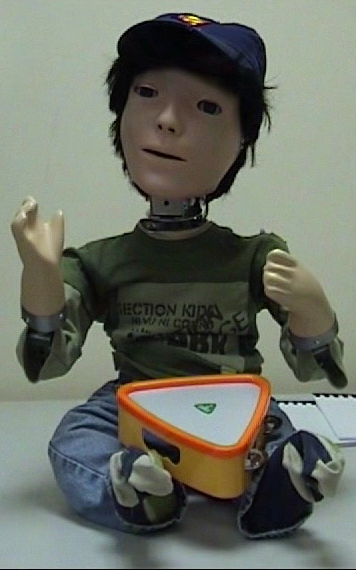
\includegraphics[width= 3cm]{img/Dautenhahn}
\captionsetup{width=3cm}
\caption{KASPAR: Dautenhahn K. et al., 2009}
\end{subfigure}
\begin{subfigure}{4cm}
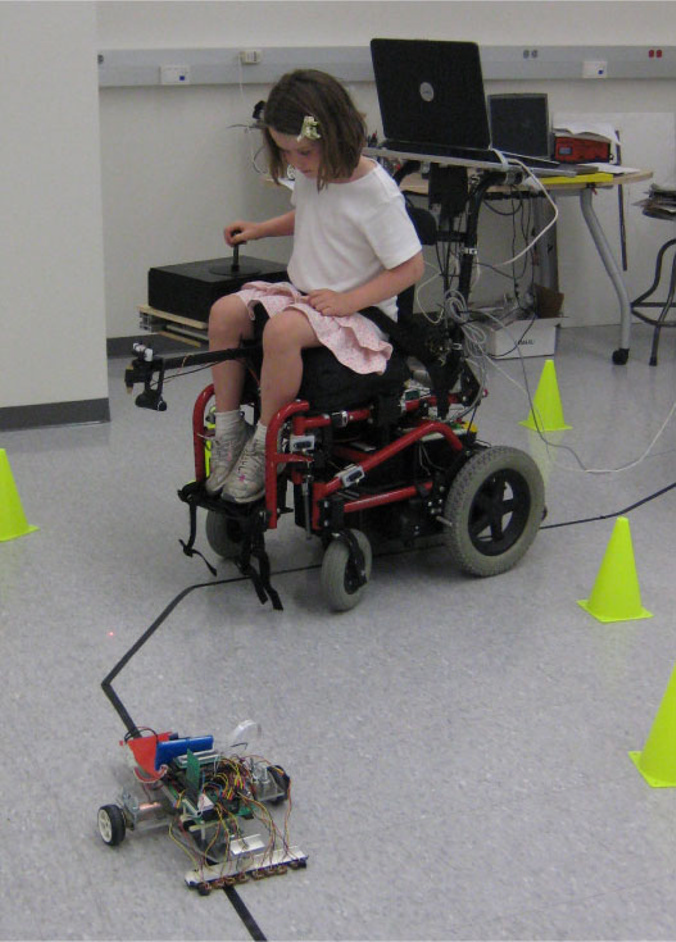
\includegraphics[width=3cm]{img/Marchal-Crespo}
\captionsetup{width=3cm}
\caption{Marchal-Crespo L. et al., 2010}
\end{subfigure}

\caption{Examples of social robots used with disabled children(2).}
\end{figure}
 
\section{Concept}

Playing is good for children, under many aspects of their development (cognitive, relational, psychological, social, physical \textellipsis). Although disabled children are deprived of this possibility more often than the others, it seems that playing would even be more productive for them.
This project aims to verify this assumption, with particular regards to the social benefits of play for motor disabled children.

We focused in particular with children with motor disabilities, although some pathologies typically affecting neuromuscular system may also result in sensitive and cognitive issues, e.g. quadriplegia, cerebellar ataxia, hemiparesis \textellipsis
In fact, up to now, the main addressees of the experiments were children with ASD, and therefore the games were designed for children who could move (in most cases) with little physical restrictions.

Little in comparison has been made for children with motor disabilities, and the employ of robotics up to now hasn't produced the same results as with children with ASD.
\\
This has 4 main reasons:

\begin{enumerate}
\item The range and severity of difficulties in movements is very wide even among patients with the same pathology, and also because of the variety of different illnesses that can result in motor disabilities
\item Often, as the game\textendash rules are extremely simplified to allow children to succeed, the game gets boring and repetitive very quickly. On the other hand, a game should not be too complicated so that the child can play freely
\item Low playfulness of patients (due to the difficult interface with the robot but especially due to the impossibility of playing with peers)
\item Complicated and time\textendash expensive interface needed in the most severe cases (such as quadriplegia) e.g. Eye Tracking Devices, Sip-and-Puff switches, head wands or mouth sticks, Voice Recognition software \textellipsis
\end{enumerate}

\section{Focus on the problem}

Since time was short to design interfaces able to deal with all of possible impairments, we needed first to select a specific target of patients.
\\
\\
\textbf{Inclusion Criteria:} We chose to work for children with medium motor impairments, and which do not have severe cognitive and sensitive problems (reserving the option to adapt the interface for other types of conditions, such as tetraplegic patients, at least in a future development\textendash perspective).
\\
\\
\textbf{Age:} 7\textendash 12 years (or mentally equal in case of cognitive disabilities).
\\
\\
\textbf{Limitations:}
\begin{enumerate}
\item the child is possibly sat on a wheelchair and may not be able to move much further from it;
\item his/her movements may be imprecise and/or sudden, he/she may not be able to calculate strength;
\item child is possibly not able to speak properly and may need time to plan the movement as he/she may not hear/see perfectly.
\end{enumerate}
\textbf{Problems to be solved:}
\begin{enumerate}
\item the game must not be boring after a few times,
\item at the same time, the game must be simple enough for the child to play even with difficulty in movements;
\item multi\textendash player possibility: the child must be enabled to play with others (whether other disabled children or not) without the game looking fake (too much advantage for the patient) or impossible to win. That is, the game should provide a way to even the possibilities of each;  
other requirements:
\item the robot must be safe for the child to handle if he/she wishes to, and possibly be satisfactory on the sensory point of view;
\item the robot should possibly give the child feedback when playing, just ad if it was a peer itself.
\end{enumerate}

\chapter{Methods}

\section{Creation of Game/Rules}


\includegraphics[width=\textwidth]{img/logo}
\subsection{The Story}

ESPer is a little owl\textendash shaped alien, employed at the PIAP Inc. (Pluto is a Planet), a company based on Volcano, in a not so far	extendash galaxy. His job is to keep an eye on some old satellites in the orbit of the planet Dab\'{o}n. These satellites are very old and sometimes their program stops working. The way to fix them is to crash Esper's pod onto their panels. The network of these satellites is owned by Sirocco Studios, that creates cartoons for children, and therefore it is very important to keep it active. When the satellite is lighted up it means it is broken and needs fixing. If the satellite does not start working again in 13 seconds, the whole network crashes and needs a whole day to be brought back to normality. ESPer is short\textendash sighted and needs help to do his job.
\\
Help ESPer keep children happy!

\subsection{The Game}
We took inspiration from pinball and bumper cars to create a game in which the goal is to drive a small vehicle onto a board in order to crash into totems that are light up randomly.

The vehicle (from now referred to as Robot) is controlled by the child with a very simple joystick, while the lighting of the totem is controlled by circuitry inside the board. The board also provides a display onto which the score and time is showed, and is fit with some barriers on the borders that prevent the robot from falling out. Both the robot and the board are fit with sound/light effects to make them appealing.
\\
\\
\textbf{Single Player Mode:} every set time, the board would decide to light up one of the five totems, and the child should try to hit it as quickly as possible. If he/she succeeds before time is over, he/she scores. The time given to complete the task is 13 seconds.
\\
\\
\textbf{Two Players Mode:} two children may play one against the other to reach the higher score by hitting totems more quickly.
(due to little time available for  design and construction, we focused only on single player mode)

In order to even the abilities of the two players, it would be interesting to program robots to randomly not execute the command from players but to go randomly around, as if it was their choice. More details about this can be find in the Robot section.

\section{Controller}

The controller represents the most interactive part of the game, for it is the connection that allows the child to express his/herself.
We developed a few ideas that should cover a wide range of possible impairments, but due to lack of time, we chose only to develop one of them.

\subsection{Joypad}
Controller with 3 very large buttons that order the robot to accelerate forward (middle button), or to spin to the left or right (left and right buttons).

\begin{wrapfigure}{r}{0.4\textwidth}
 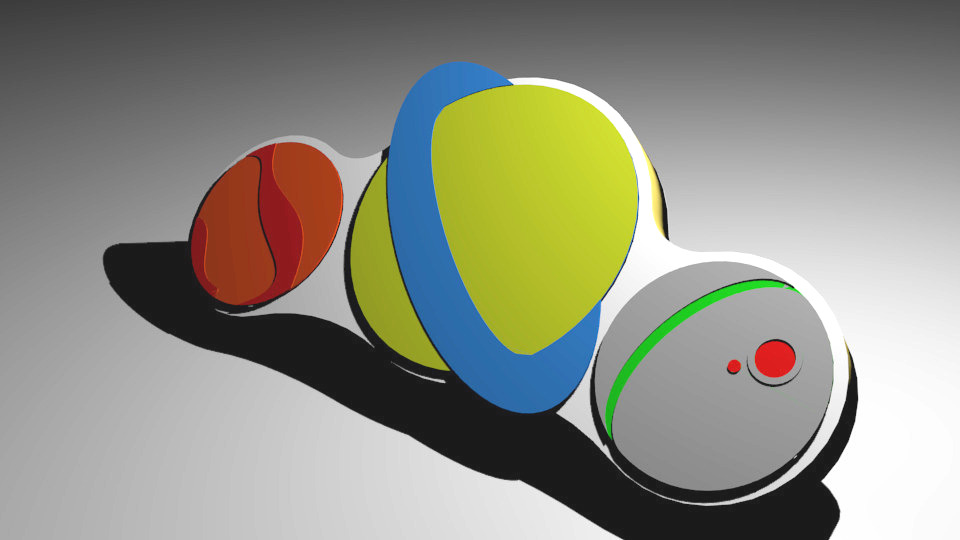
\includegraphics[width=6cm]{img/joypad.jpg}
 \caption{3D render of the joypad}
\end{wrapfigure}

The joypad may be set on the table with the board or secured to the wheelchair armrests using straps.
\\
\\
\textbf{Advantages:} this type of controller offers the possibility to patients affected by distonia or spasms to drive the robot without accidentally hitting the wrong buttons. It also can be decorated easily and provided with sounds or lights to make it more appealing, since it is quite large (approximately 50cm wide)
\\
\\
\textbf{Disadvantages:} not suitable if the patient is unable to reach the correct position to press the button (because of spasticity or paresis) or if is very weak, so that he/she tires easily.
This controller was not developed because of lack of time and materials needed.

\subsection{Accelerometer Wrist/Head Band}
\label{ssec:accel}
Wearable controller that can be tied to the child's wrist. The controller is simply an accelerometer and a control circuit that allows the patient to spin the robot on the left or right by swinging the arm (in this case the robot moves forward by itself).
\\
\\
\textbf{Advantages:} useful for patients who cannot reach the joypad/joystick or are too weak to push the buttons.
\\
\\
\textbf{Disadvantages:} may be still not useful if patient is tetraplegic or affected by spasm and sudden movements. Moreover, the use of accelerometers requires an accurate signal analysis. This is especially true when considering the filtering needed to adapt the interface to the movements of the patients, which can be imprecise, jittery or discontinuous. 

Therefore, because mainly of lack of time, we chose not to develop such a controller, but it stands as a future development, in the perspective to create multiple interfaces that can cover the widest range of possible impairments.

In the case the patient is tetraplegic, the controller can be adapted to fit on the forehead too (just as if it was a head wand), but in this case the patient may get tired easily.

\subsection{Joystick}

Very weak children may not be able to swing/push the controller long enough to play effectively. If they have sufficient control over at least one upper limb, it is possible to create a joystick. It is sensitive enough to allow the patients to drive the robot without tiring, and has four positions: forward, backward, left and right. There should be also a ON/OFF switch and a slot for batteries. Joystick and its shell are smaller than the joypad and can be positioned where the patients can reach it without difficulty (using straps).
\\
\\
\textbf{Advantages:} can be fit onto wheelchair's armrests, just like normal controls of a scooter. These patients are very practical in driving their scooters and therefore they should fare well with such an interface. It does not need strength.
\\
\\
\textbf{Disadvantages:} the patient needs control over one arm at least. Therefore it is not suitable for tetraplegic or distonic patients.
\\
\\
We chose to develop the joystick for it looked more immediate, since it resembles a well\textendash known interface for wheelchair driving patients.
\\
\subsubsection{Mechanical part}

The shell provides protection for electronics, support for the joystick and on/off button, and access to battery slot. The shell was realized partly modifying a wooden box, and partly by building pieces ourselves. The shell should not be too large as it needs to be placed ideally besides the wheelchair's armrests, and should not hamper the child's movements.
The lid of the shell is made up of two parts:

\begin{itemize}
\item a sliding part that can be easily moved and allows to change batteries (which is the part the user should have access to);
\item a fixed part that covers circuitry and provides support for the joystick, button and LED. This part can be removed by screws, so that control unit program or circuitry can be modified, but should not be accessible to children.
\end{itemize}
The joystick is secured to the fixed lid with screws.

\subsubsection[Electric part]{Electric part \footnote{For the electric scheme, see \autoref{app:circuit}; for implementation information, see \autoref{sec:software} and \autoref{app:code}}}
Requirements of this part are: 
\begin{itemize}
\item provide power;
\item interpretation of the inputs given by user (direction of the robot and pause);
\item transfer data to board and receive from it (or from/to robot);
\item give sensory feedback on the state of the controller;
\end{itemize}
The circuitry is powered by 3 regular 1.5V AA batteries, provided with their battery slot. We made this choice basing on the ease to find the batteries, size, and possibility to recharge them. Control unit (ESP12) receives right input voltage from 3.3V regulator (AMS1117), that also provides power to Op\textendash Amp (LM378) and analog MUX (PC74HC4053)
\footnote{For more information about ESP, see \autoref{app:ESP}}.
The choice was made mainly on order to give the ESP a regulated tension, that should remain stable for a while also when the batteries start running out.

Since the FSR (Full Scale Range) of the ADC on control unit is only 1V, a trimmer connected to the actual joystick reduces power to proper value. The joystick consists of two potentiometers (one for axis and one of y axis), each a $5k\Omega$ resistor.
The trimmer value is decoupled by a buffer, then given as input to the actual joystick (which is standard for ARDUINO interfaces). The outputs are given to the MUX, which is controlled by ESP12 that selects inputs from the two axes alternately. Output is then given to ADC input of ESP. The decoupling by the buffer is necessary for otherwise the tension given to the MUX would not depend only on the potentiometers, but also on the. This way we ensure a stable voltage supply for the potentiometers. 
The joystick also provides a button (which is activated by pushing the joystick down). This input is given directly to ESP and serves as a \textquotedblleft everything button \textquotedblright, allowing the user to pause and resume the game, even if he/she cannot reach the everything button on the board.

The circuit is switched on by a spring button switch connected directly to the battery slot. A red LED light signals when power is on, and a RGB LED (blue) signals when the ESP is online. The frequency of the blue LED flashing identifies the state of the controller at the moment:
\begin{itemize}
\item idle \textemdash doing nothing: off;
\item scanning \textemdash searching for available networks: slowly blinking;
\item connecting \textemdash attempting connection with suitable server on the network: fast blinking;
\item standard game mode \textemdash connected to board and ready to play: alternatively fast and slow (this does not change when game is paused);
\item standalone mode \textemdash directly controlling the robot: no blinking.
\end{itemize}


\subsubsection{Positioning}

In order to place the joystick comfortably, we realized a strap (made out of Velcro), that can be tied to the wheelchairs armrest. A complimentary Velcro is glued to the bottom of the joystick shell in order to ensure adjustment of the positioning. 

There are two possible configurations, depending on the mobility of the child: the strap can be either wrapped around one armrest (for example, behind the scooter controls), or fastened across the space between the two armrests, so that the box can be placed in the  middle. With this system, though sacrificing some stability, we ensure a wide range of positions that can be reached by the patient.

\subsection[Virtual Interface]{Virtual Interface \footnote{For implementation information, see \autoref{sec:software} and \autoref{app:code}}}
In order to test and debug the game while work was still in progress, we created a graphic interface that can simulate both the totem system (with display) and the joystick. From this interface we created a simplified version of joystick that could be used to adapt the controller to different users. By creating an actual virtual controller, the child has the possibility to use his/her own tablet or laptop to play. Patients with most severe restrictions are often provided with personal computer interfaces (e.g. to drive wheelchairs) and a controller application would represent an immediate and flexible approach in order to broaden the range of suitable users.

\section{Robot}

The second most interactive part of the game is represented by the robot (ESPer). If the controller allows the child freedom of expression, the robot is the part that deals with him/her as a peer. 
\footnote{For implementation information, see \autoref{sec:software} and \autoref{app:code} }
\\
It consists of three main parts:
\begin{itemize}
\item frame (that supports and protects the circuitry and shell), and wheels;
\item electronics: batteries, regulation circuitry, lights, motors, control unit;
\item outer shell (or \textquotedblleft head \textquotedblright) that can be decorated to form a personalised\textquotedblleft outfit \textquotedblright and provides further protection for electronics;
\end{itemize}
It receives instructions from the controller through wi-fi connection. The wireless network developed allows the child to control the robot with the controller independently from the board: if the robot sees the board activated, it connects with it and the game can start (standard game mode), while if the board is not active (its network is not on), the robot can used alone (stand alone mode). We chose to create also this second mode in order to allow the child to use the game even when the board is charging batteries, or if the board set-up is made difficult, due to its dimensions. In this mode the robot can be used on the floor as well.

The batteries are accessible by removing the outer shell from the top of the robot. To prevent the user from touching the circuitry inside, the batteries are stored in a separate section of the robot and only the connectors are accessible.
Ideally, the best approach would be to have the batteries placed on the bottom and removable using their own slot, without having to remove the outer shell. This was not done due mainly to lack of material.

Moreover, the robot needs to be small enough to move freely on the board (approximately 7cm in diameter). The problem of the size is particularly pressing when approaching the corners of the board, for the space left between edges and totems is very narrow. This is due mainly to the size of the wheels. To reduce the effect of this, the robot is programmed to stop progressing while the bumper is pushed. That is: the robot ignores the command \textquotedblleft forward \textquotedblright while it is pushing against and obstacle and only turns on the spot to avoid it.

\begin{figure}[b]
 
\begin{subfigure}{0.5\textwidth}
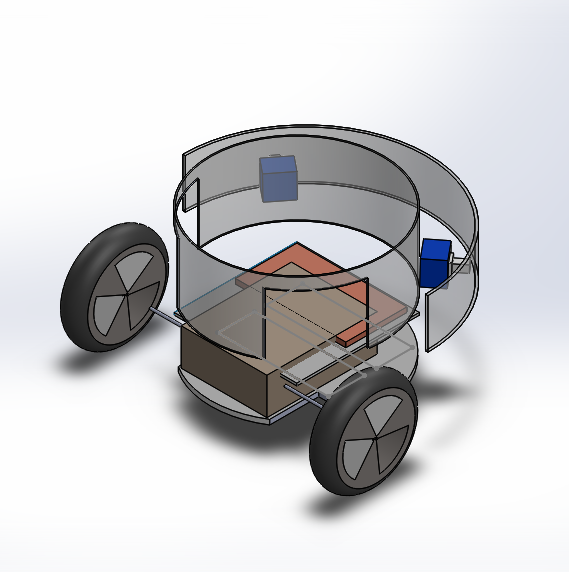
\includegraphics[width=0.9\linewidth]{img/robot} 
\end{subfigure}
\begin{subfigure}{0.5\textwidth}
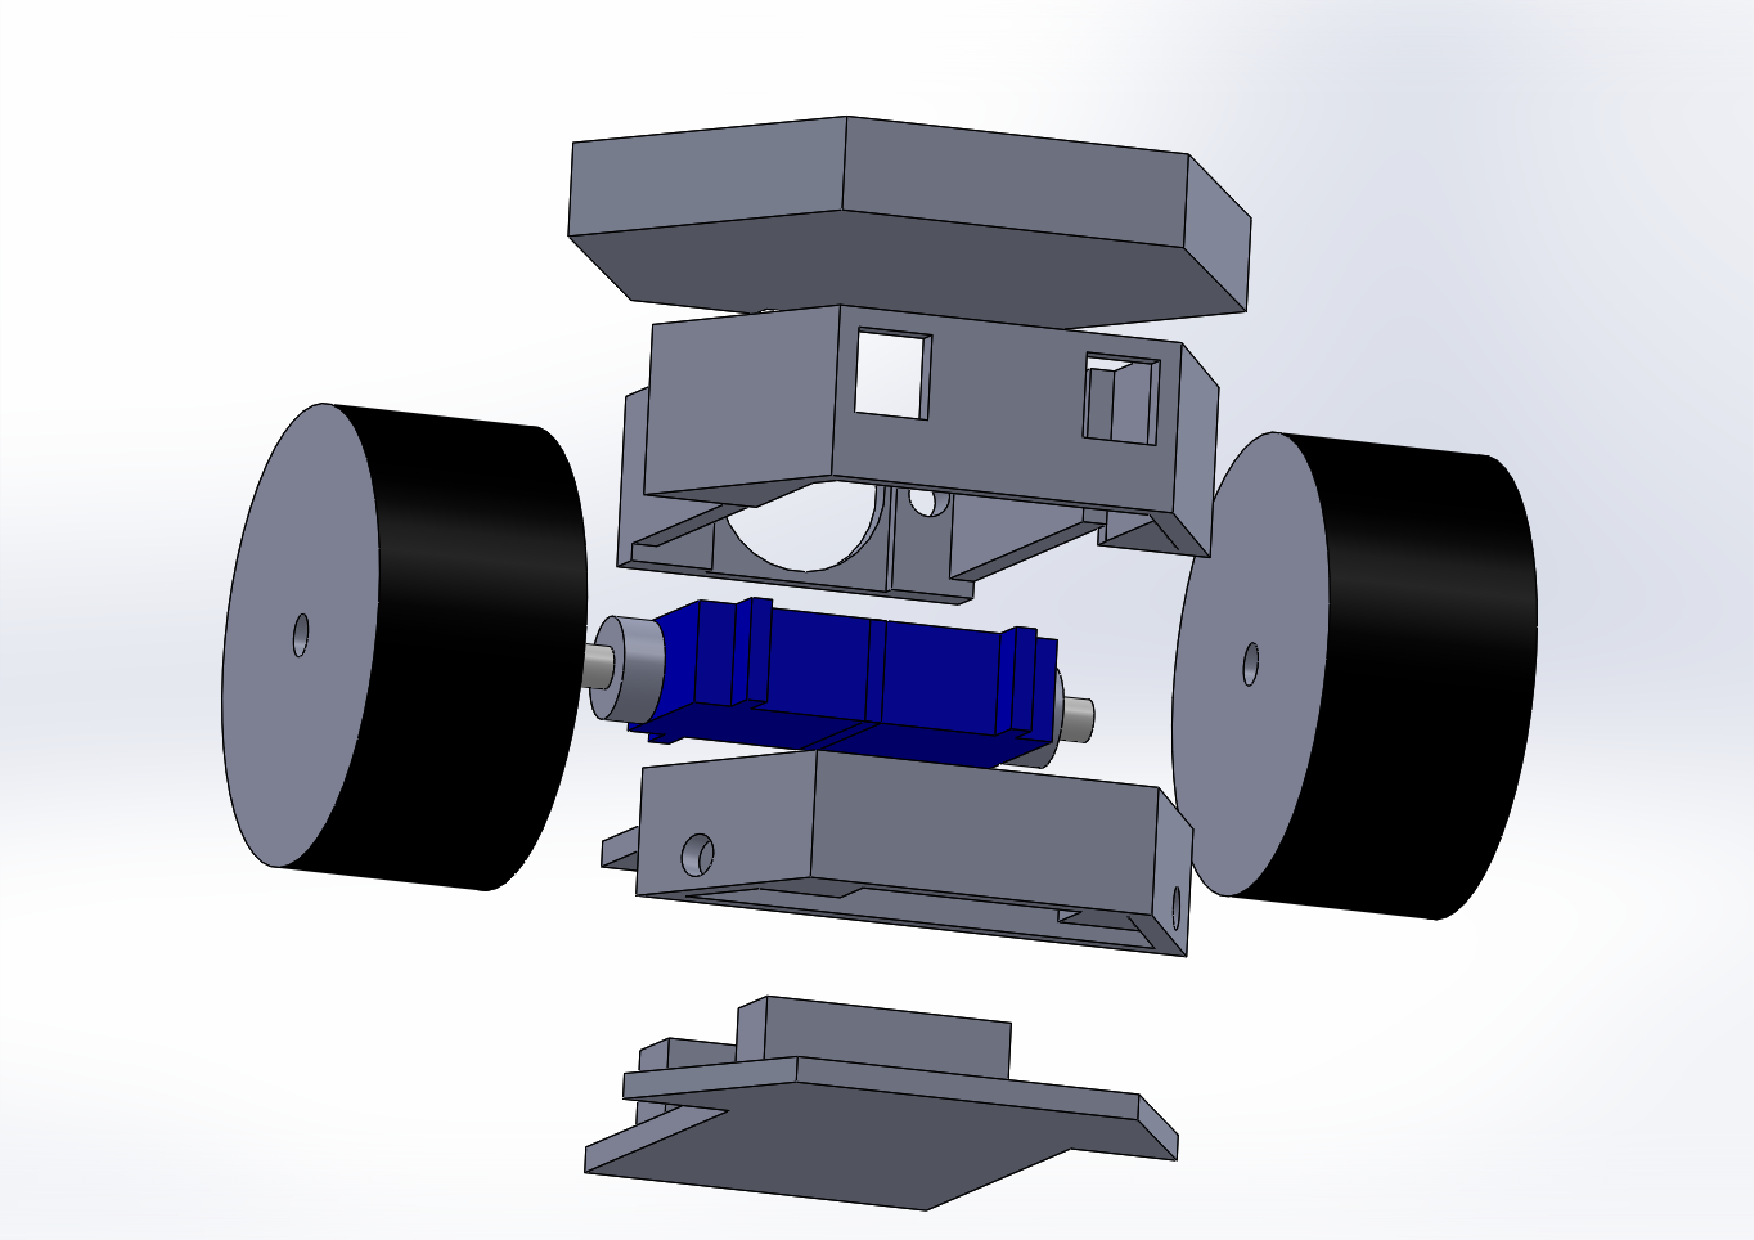
\includegraphics[width=0.9\linewidth]{img/robot1}
\end{subfigure}
 
\caption{CAD models of the inner structure of the robot.}
\end{figure}

\subsection{Frame}

The frame consists of a round plastic basis and a carton cylinder. On the basis are secured the motors and circuitry onto which are placed batteries. There are LEDs on the cylinder (green and red).

On the side cylinder also there are two switches covered by a plastic plaque that form the bumper, and the ON/OFF switch on the back.

On the bottom part, the motors are directly connected to wheels and there is a small metal sphere secured on the front part of the robot to prevent it from tilting forward. The motors are actually servomotors that have been modified so that they can spin at 360\degree. This is due to lack of time, poor information supplied by data\textendash sheets on online markets, and cost of components. This arrangement causes the two motors not to spin at the same rate, so that it may be useful to verify that this problem does not affect manoeuvrability too much. Anyway, considering the size of the board (70cm) and placement of totems, the robot needs not to move on straight line for more than 30cm, so that we can accept some deviation without the game to suffer from this.

On the other hand, an advantage of using servomotors is that speed con be selected directly from the control unit, with no need for a driver.

To simplify the game, we chose to set the wheels only to spin at one speed, both clockwise and counter-clockwise. Steering is achieved in two different ways, depending on the inputs from the controller (in this case, the joystick):
\begin{itemize}
\item by blocking one of the wheels, so that the robot turns while progressing (either forward or backwards). This corresponds to tilting the joystick to upper/lower left and to upper/lower right;
\item by spinning the wheels in opposite directions, so that the robot turns on the spot. This corresponds to tilting the joystick to the left or right;
\end{itemize}

\subsection{Electronics}

\begin{figure}[h]
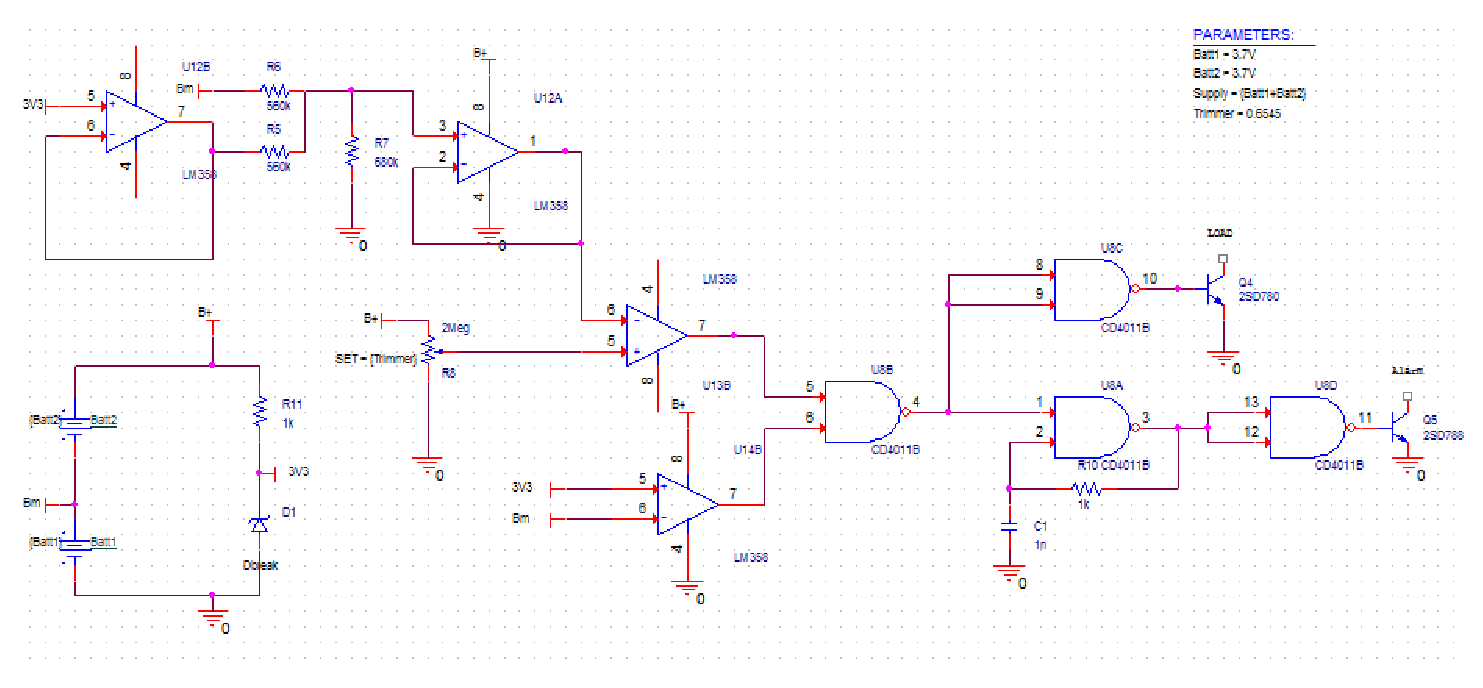
\includegraphics[width=\textwidth]{img/ProgettoCircuito.eps}
\caption{Electric scheme of robot circuitry}
\label{fig:robot_circ}
\end{figure}

The robot is powered with two 4.7V LIPO batteries, and can be switched on/off through a switch on the rear part. We chose to use LIPO batteries because, although more expensive, they are rechargeable and \textemdash compared to the alternatives (such as Stilo) \textemdash provide a better \textquotedblleft power-to-bulk \textquotedblright ratio, for they are lighter and smaller than the others.
The control unit (ESP12\footnote{For more information about ESP, see \autoref{app:ESP}}) requires 3.3V input voltage, given by the same regulator used in the controller (AMS1117).

The circuitry also provides a way of monitoring the voltage of the single battery through two triggers. When one of the two batteries drops below a threshold (set at 3.3V), the circuit cuts them off from the rest of the more power-consuming electronics (such as motors), preventing degeneration of batteries. The circuit provides connections between motors, LEDs, and bumpers, and ESP12 as well as access for programming.

The circuit was designed entirely by us and printed as PCB by a Chinese manufacturer.

\subsection{Head}

The role of the outer shell is mainly decorative, but is it also useful to dampen impacts and protect the inner part. In this case, we gave Esper a colourful look to appeal kids, and to ease realisation but also more \textquotedblleft technological\textquotedblright outfits could be considered, such as space saucers etc. This is particularly true if we consider the possibility to play with another child, so that the two ESPers are recognizable.
The shell consists of a papier\textendash m\^{a}ch\'{e} mask under a painted striped tissue cover fitted with an elastic band. There are also a couple of antennae that can be bent as one pleases fixed on the head. These were realised in metal wire and wool.
Ideally, the outer shell could also provide sensory feedback for the child, in case he/she wishes to handle it.
This requires also the frame to be robust. Unfortunately, we had to neglect this side, due to lack of time/materials but especially owing to the need to continuously revise the circuitry and programming. Therefore the head is designed more to be easily removable (also because the batteries are accessible only from above) than to be sturdy.

\subsection{Interaction and Feedback}

Being responsible for an important part of interaction with the patient, it should have a range of sound/lighting effects.
\begin{itemize}
\item red and green LED lights (2 couple) that signal the state of the robot, like they are used in the controller;
	\begin{itemize}
	\item \textbf{idle} red on, green off;
	\item \textbf{scanning} searching for available networks: red on, green slowly blinking;
	\item \textbf{connecting} attempting connection with suitable server on the network: red on, green quickly blinking;
	\item \textbf{standard game mode} connected to board and ready to play: red and green alternately blinking (this does not change during the pause);
	\item \textbf{standalone mode} directly controlling the robot: red and green both on.
	\end{itemize}
\item Buzzer that emits sounds when the robot crashes, etc. We decided to delegate this part to the board as well, for the RPi can control the buzzer more efficiently than the ESP in the robot, providing more effective interaction, although sacrificing realism.
\end{itemize}
In a future development perspective, it was our intention to give the robot the possibility to disobey the user's commands from time to time, and randomly act on its own decision. This should not be as if openly helping the disabled child (in case the other player in not disabled).

It also should give the impression that the robots have actually their own will, but are not capable of doing thing on their own, so that the child perceives that he/she must help them (in the story, we justify this by saying that ESPer is short-sighted). We believe this is very important to develop self-confidence and social skills.

The sounds from the robot are provided by the board, and they are divided according to the situation in which they occur:
\footnote{See also \autoref{app:noise}}

\begin{enumerate}
\item entering the game from main menu;
\item resuming the game from pause menu;
\item scoring (hitting the totems);
\item running out of time (last 5 seconds of time allotted, when the totem starts flashing);
\item failure (not hitting the totem in time);
\end{enumerate}


\section{Board}

The board offers mechanical support the robot and totems, as well as central control unit and Wi-Fi network connection. Also, it provides lighting and sound effects to the whole interface and it is decorated accordingly to the theme.
\\
It consists of three main layers:

\begin{itemize}
\item top layer, that can be open to operate on inner circuitry, and in which there are holes for the totems and for the removable boundaries. It is punctuated with white LEDs to mimic a starry sky, and it is covered by black plastic to simulate background;
\item middle layer, that creates the room for inner circuitry and power supply and creates the connection between the sections;
\item bottom layer, that provides basis for the totem mating and onto which middle layer is secured.
\end{itemize}
The display for scoring is located on the sides, as well as LEDs signalling the state of game, ON/OFF switch, and the \textquotedblleft everything button\textquotedblright. On the top there are also small holes that show the battery charge (being located above the battery pack).


\begin{figure}
\centering 
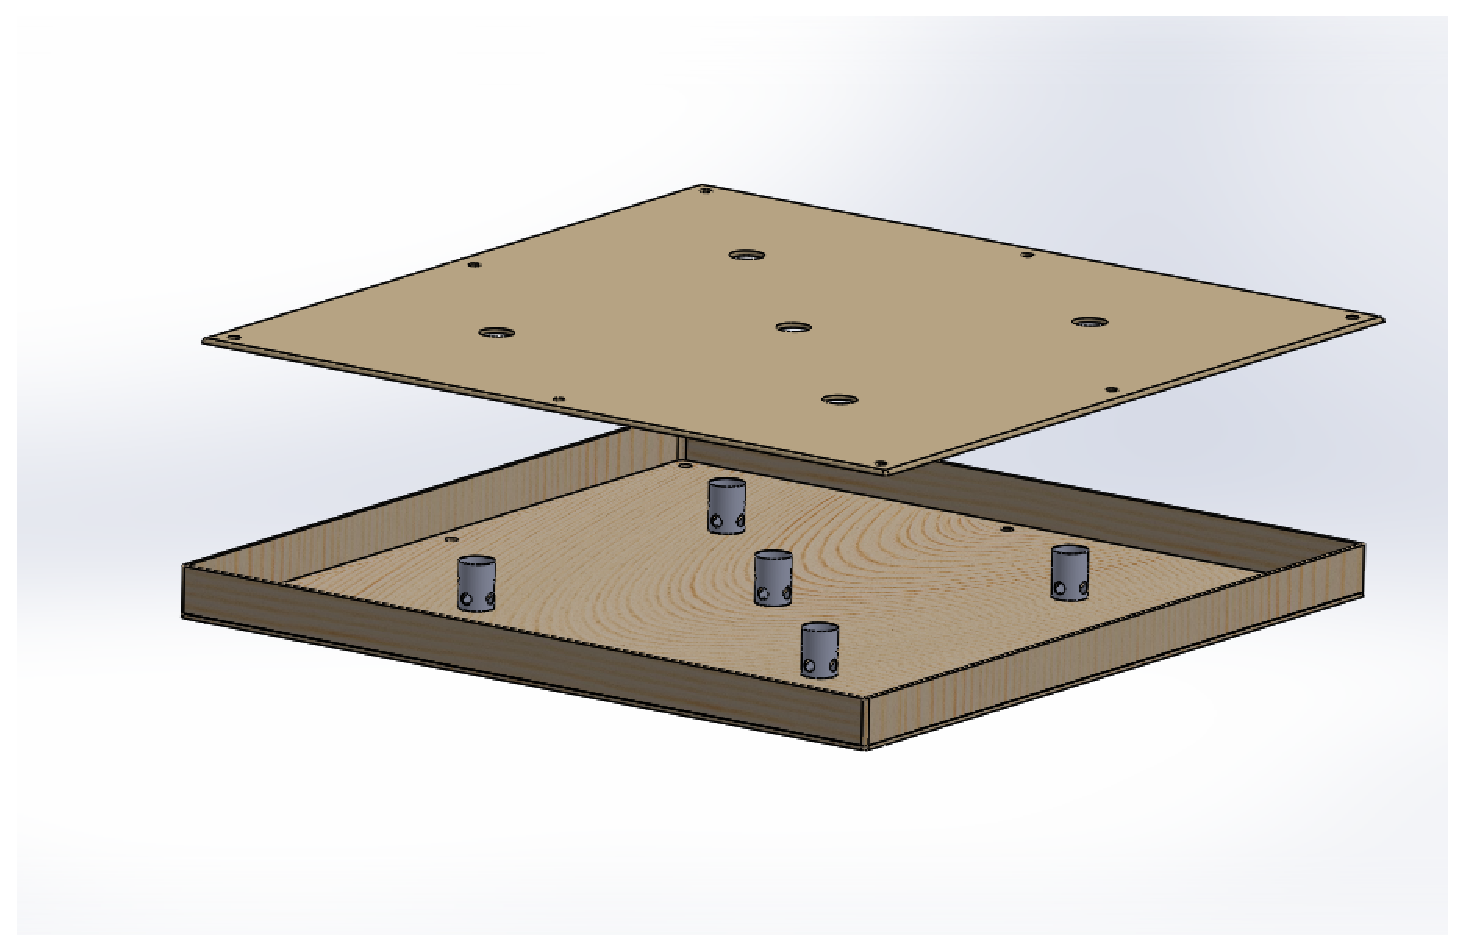
\includegraphics[width=0.9\textwidth]{img/BoardVistaInsieme3.eps}
\caption{CAD of Assembled board (top removed).}
\end{figure}

The board was designed to be divided in four quarters that could be disassembled and transported more easily. The pieces are not the same size because of the middle totem: it would have been extremely difficult to create the basis for the  mating if we had had to split it into fourths.

When assembled the body is 70x70cm wide and the thickness (mostly made up by middle layer) is about 5cm.

The sections are made out of lightweight wood and plastic and are connected with each other:
\begin{itemize}
\item mechanically (through wooden nails);
\item electrically (through 4 channel 3.5mm jack plugs);
\end{itemize}
In order to ease the use of the game, all the circuitry and control unit (Raspberry Pi or RPi\footnote{For more information about Raspberry Pi, see \autoref{app:RPi}}) are located in the largest plaque (the one with two totems), from now referred to a \textquotedblleft main section \textquotedblright.

The main section contains also a battery pack and a pin (micro USB) to access it. This ensures the RPi to receive its proper input voltage (5V) and that the board can be recharged without extracting batteries but simply by plugging in the main section.

Moreover, this way the entire game could be played with power provided directly from electric distribution (for the battery pack does not need to be disconnected to be recharged, unlike LIPO batteries).

There is also another jack input to connect to game to an audio system (e.g. headphones, speakers \textellipsis). The board on its own does not provide sounds if not connected to external device. Since it is lacking its own volume regulation, this allows the user to adjust it to his/her own preference, or even to exclude completely the audio.

The main section receives information from all other game components (robot and controller) via Wi-Fi, and from the totem via cables.

We chose Wi-Fi over other type of connections (e.g. Blue-tooth) for:
\begin{itemize}
\item ESPs and RPi provide built-in Wi-Fi connection;
\item Wi-Fi connection is supported by a wide range of devices: laptops, tablets, cellphones \textellipsis while others may not always be. 
\end{itemize}
The drawback is that this kind of procedure is more energy consuming compared to Blue-tooth, for example.
The RPi is responsible for collecting this information, processing it and sending it back.
\\
These processes include:
\begin{itemize}
\item detecting the impacts between totems and robot;
\item updating the score and reset when needed;
\item lighting totems;
\item counting time to the next target;
\item transfer information from controller to robot;
\item management of display;
\item management of sound effects\footnote {See \autoref{app:noise}} (when connected to output).

\end{itemize}
The implementation needed in this process is extensive and so we describe in a separate chapter\footnote{ See \autoref{sec:software}}.
Battery pack, RPi and circuitry are secured into their positions by screws and metal bands. All pieces contain the basis for the mating with the totems (described in the totem section).

The board also provides some boundaries to prevent the robot from falling off the top. They come in the form of wooden planks (5cm wide) with hinges that allow them to be folded and stored. They are secured to the top layer by wooden nails as well.

\begin{figure}[h]
\centering
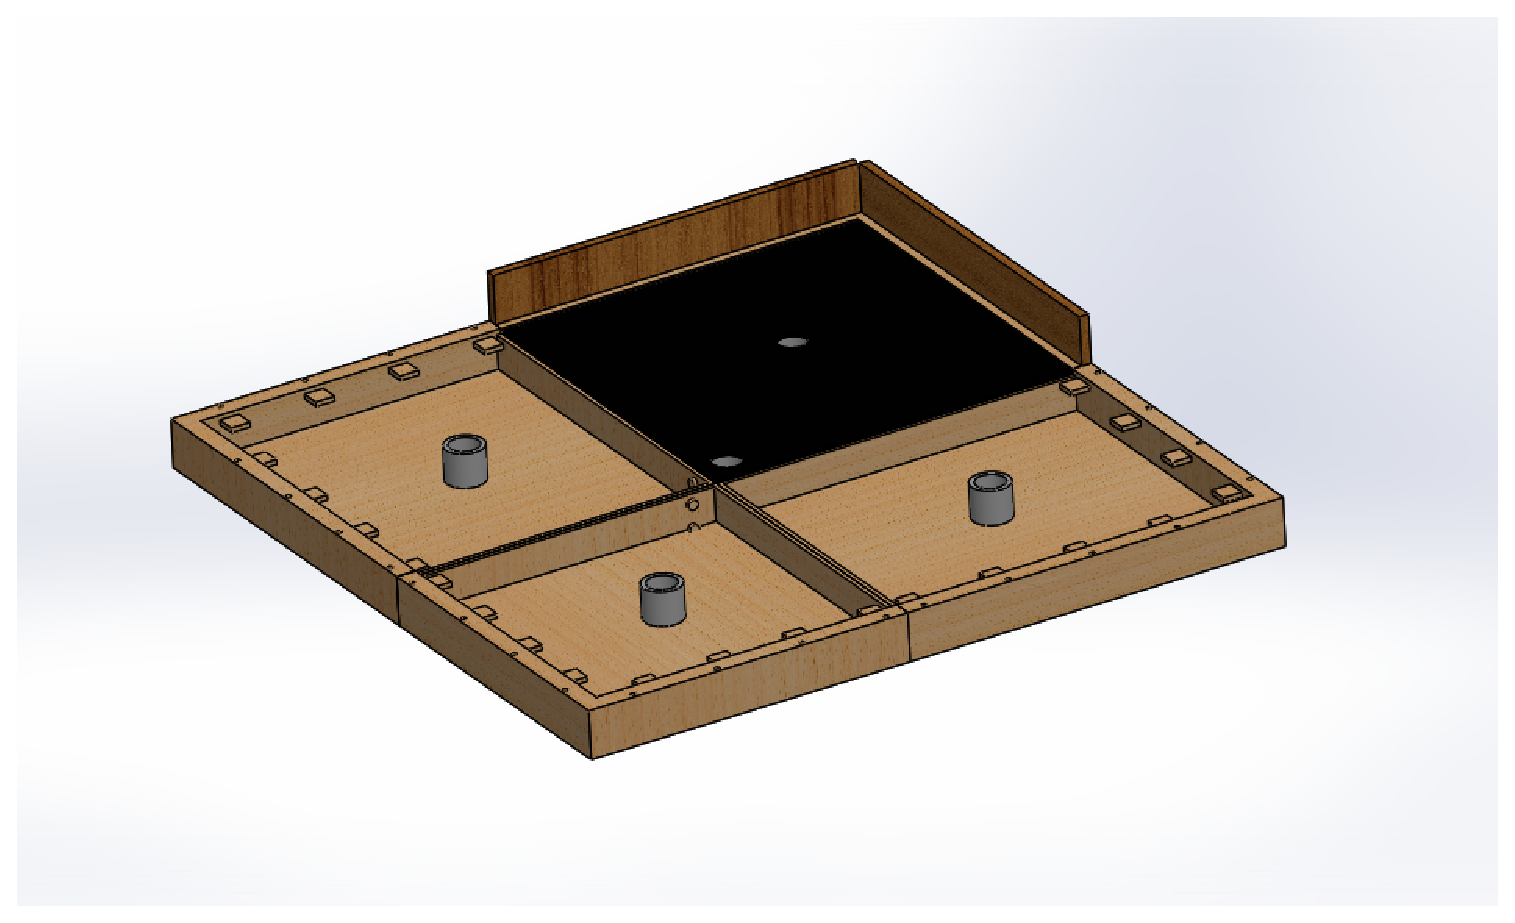
\includegraphics[width=0.9\textwidth]{img/Board.eps}
\caption{CAD of Assembled board with detail of section.}
\end{figure}

\subsection[Display]{Display \footnote{For details on implementation, see \autoref{sec:software} and \autoref{app:code}}}

The display is a LTC4727G 7-segment common cathode, with four digits and seven points. It is controlled directly by ARDUINO UNO\footnote{For more information about ARDUINO, see \autoref{app:Arduino}}, that receives serial instructions from RPi. This is because, having many processes concurrently running, the Raspberry Pi does not manage to control the display most effectively, so that it tends to flicker quite visibly if directly controlling the display.

Apart from keeping track of the score and time countdown, the display is also used as a way to give more information about the game state and to improve appearance, contributing to the \textquotedblleft space adventure \textquotedblright atmosphere.

For example, the display shows \textquotedblleft FlipperBot \textquotedblright sliding from right to left in the main menu, or \textquotedblleft LOSE \textquotedblright when time runs out, as well as some animations in between the various states.


\subsection{LEDs}

There are three lights:
\begin{itemize}
\item ON/OFF LED \textemdash red light signalling when the board is turned on;
\item Player LEDs \textemdash two yellow LEDs lights, one for each player. The state of game is represented by the frequency of flashing:
	\begin{itemize}
	\item LED is off \textemdash both controller and robot are not;
	\item LED is on, no blinking \textemdash both robot and controller are online, ready to play standard game mode;
	\item LED slowly blinking \textemdash robot is online, but not controller;
	\item LED blinking fast \textemdash controller is online, but not the robot.
	\end{itemize}
\end{itemize}

\subsection{The \textquotedblleft everything button\textquotedblright}

The big round button besides the ON/OFF switch allows the child to:
\begin{enumerate}
\item start the game \textemdash by pushing once from the main menu (that starts automatically when turned on and to which the player returns in case of loss);
\item pause the game \textemdash by pushing once from the game session. This stops the countdown and disconnects the robot;
\item resume the game \textemdash by pushing once from pause menu;
\item return to main menu \textemdash by holding the button 3s at least during pause.
\end{enumerate}
All of these passages are supported by the change in music themes 
\footnote {See \autoref{app:noise} for more information}.


\section{Totems}

Totems are the targets into which the robot must crash in order to score.

They consist of cylinders containing the light set and switches (to detect impacts through plaques). The outside of the cylinder be decorated accordingly to the theme (e.g. as a satellite as we chose). In order to move the game more comfortably they are designed to be easily removable from the board.

\subsubsection{Mechanical Part}

\begin{wrapfigure}{r}{0.3\textwidth} 
    \centering
    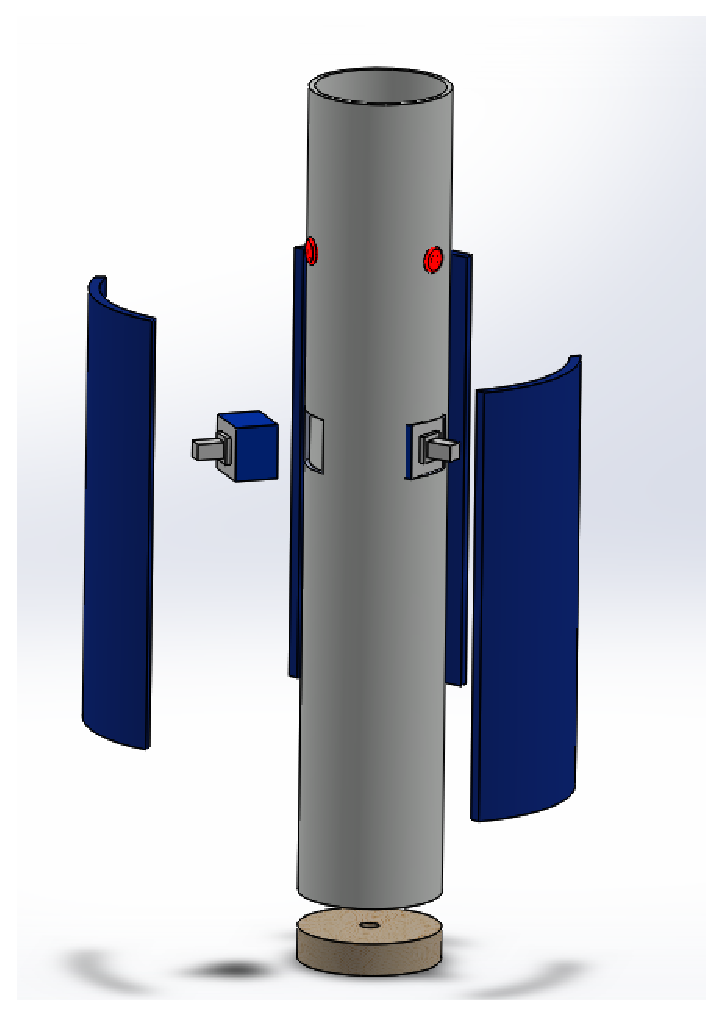
\includegraphics[width=0.3\textwidth]{img/totem_nuovo1}
    \caption{CAD model of the struction of totems.}
\end{wrapfigure}

The core consists in aluminium cylinders (inner diameter 2cm). On the lower part of the core, there are three tough plastic plaques. The plaques transfer impact to the switches to which there are connected.

On the upper rim of the core three LEDs are positioned in the upper half of the structure and provide colour and feedback (two sets are blue, two are red and one is green).
\\
\\
\subsubsection{Electric Part}
LEDs sets signal the totem that is active in that moment, and blink when the target is hit. The target blinks faster and faster as time left runs out. In the menu mode, totems are lit in a circle, waiting for the user to push the \textquotedblleft everything button\textquotedblright.

Lighting is controlled by the board onto which they are plugged, so totems do not need complex circuitry. The electronic part includes the contacts for the switches and LEDs (which are lighted up by RPi through a simple pull-up resistor) and power supply.
\footnote{For the electrical scheme, see \autoref{app:circuit}}
\\
The choice to defer the control of the lighting to the board is preferable for:
\begin{itemize}
\item there is little space to work with inside the totem;
\item allows saving of materials;
\item allows to modify easily the connection if needed by operating only on the main section (for the board collects everything there).
\end{itemize}

\subsubsection{Mating}

The mating provides ease of use, mechanical stability, electronically safe connexions. These are ensured by using the same 4 channel 3.5mm jack plugs as used to connect the board sections. They are stiff enough to ensure the totems do not tilt when hit by the robot. Moreover, they are quite a common component, so it is easy to find and replace them if needed.

\begin{figure}
    \begin{subfigure}{6cm}
    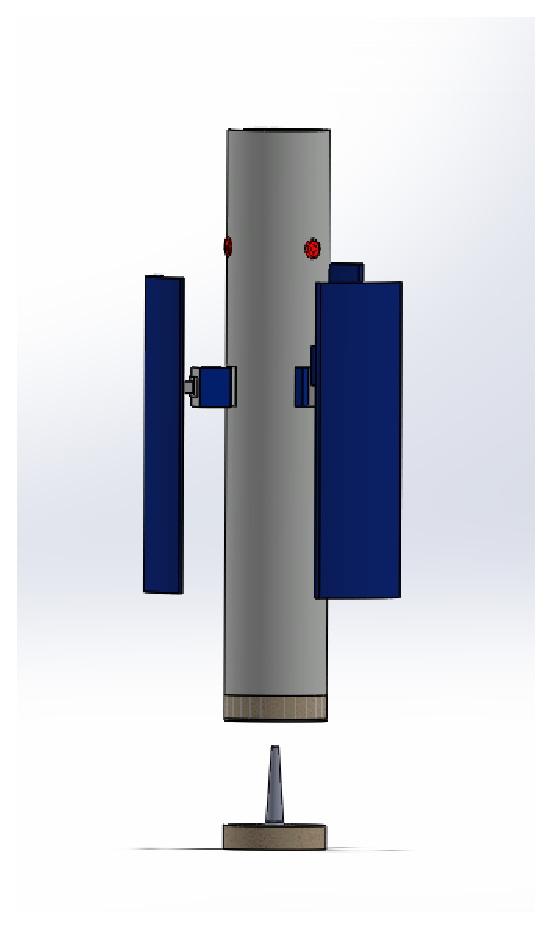
\includegraphics[width=5cm]{img/totem_nuovo2}
    \captionsetup{width=4cm}
    \caption{Model of totems with mating}
	\end{subfigure}
	\begin{subfigure}{6cm}
    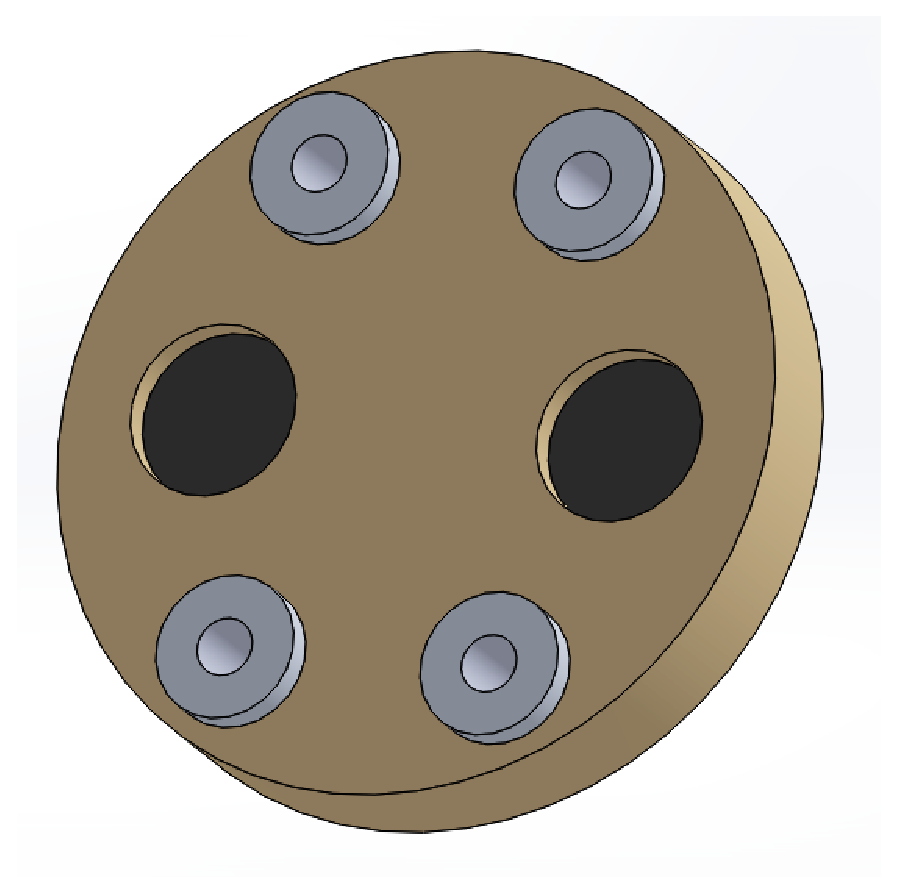
\includegraphics[width=5cm]{img/placca_contatto}
    \captionsetup{width=4cm}
    \caption{Detail of the magnetic contact plaque.}
    \end{subfigure}
\end{figure}

Further stability is provided by a cylinder of though plastic secured onto the bottom of the board, that prevents tilting and accidental contact among other wires in the board section. The complimentary plug is glued to a wooden disc from which the wires are gathered to be sent though connections to the main section.

In a future development perspective, it would be interesting to develop a mating system that should allow the child to insert the totems him/herself. We designed an alternative based on magnets:
two complimentary plaques would be fixed to the totems and board bottom. They would contain:

\begin{itemize}
\item \textbf{Magnets}: 2 small button magnets (6mm diameter) with opposite polarity. When totem is connected, only appropriate orientation (corresponding to the complimentary magnets on the board) would allowed;
\item \textbf{Electric contacts}: The connection would be provided by small screws and flat nuts for two contacts, while for the other two contacts it would be possible the magnets themselves.
\end{itemize}
On the board the corresponding plaque would be secured to the bottom layer. The plaque is lightly raised so that wires from the contacts can be gathered together and transferred to the pins, as with the current solution.

We tried to realize one of this plaques, but we had significant contact losses, especially when the totem was hit, for it tended to tilt and rotate. This is due to the facts that the magnets were not perfectly in contact, and also to the not exact alignment of the nuts. This is mainly dued to the availability of technical means we had, since this mating requires such a precision we cannot reach with manual construction alone.

On the other hand, this development is potentially very interesting, since the child is provided with the possibility to assemble part of the game him/herself, and guided in a way that does not seem to facilitate him/her excessively (for the intervention of magnets is less apparent than, say, guiding lines traced on the core that point to the right orientation). This is very useful to give the child self confidence in his/her manual ability.

\begin{figure}[h]
 
\begin{subfigure}{0.5\textwidth}
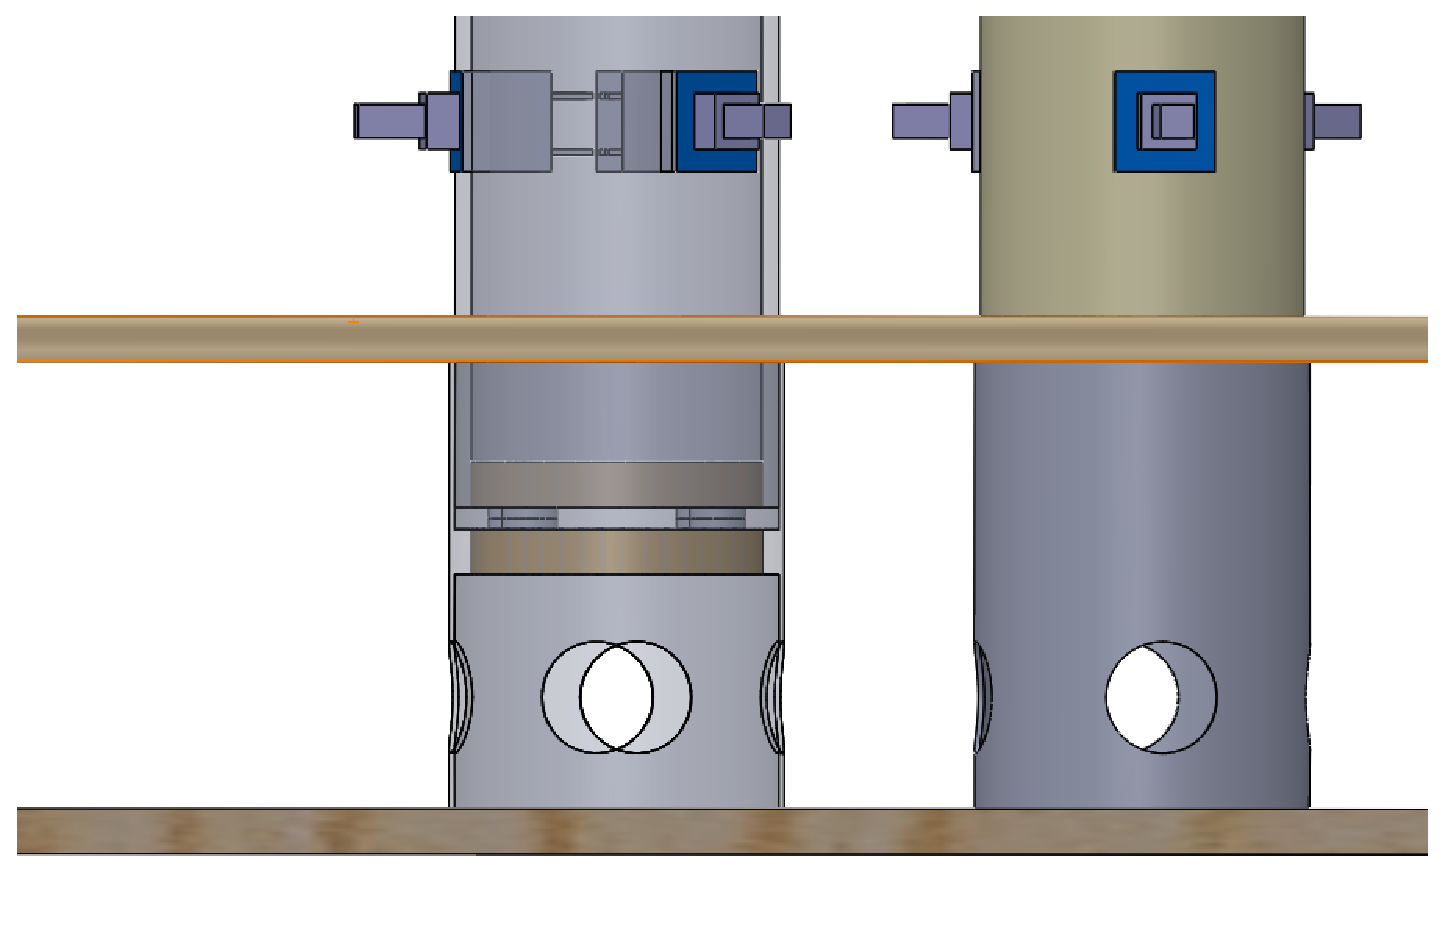
\includegraphics[width=0.9\linewidth]{img/DettaglioConnesioneTotemBoard}
\end{subfigure}
\begin{subfigure}{0.5\textwidth}
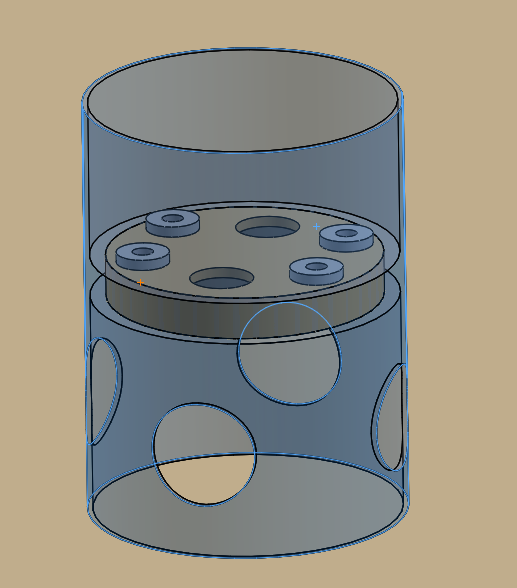
\includegraphics[width=0.9\linewidth]{img/DettaglioConnesioneTotemBoard1}
\end{subfigure}
 
\caption{Detail of the magnetic mating.}
\end{figure}

\section{Software}
\label{sec:software}
In addition to designing and building the physical parts of this
project, a considerable amount of work was put in developing the
software needed to make the various devices operate as wanted.

The main programming languages used were C++ and Python, with some
utilities written as Bash scripts.

\autoref{fig:softtree} shows the main software components of this project,
ignoring the utility tools only used during development.

Snippets of the code contained in this project can be found in
\autoref{app:code}, presented as examples of use of the various tools.

\begin{figure}[htbp]
  \import{fig_softtree}
  \caption{Structure of the main software components of this project}
  \label{fig:softtree}
\end{figure}

\subsection{Scheduler Module (\ScheMo{})}
  \label{ssec:schemo}
  \import{ssec_schemo}

\subsection{Network topology}
  \label{ssec:network}
  \import{ssec_network}

\subsection{FlipperBot Communication Protocol (FBCP)}
  \label{ssec:fbcp}
  \import{ssec_fbcp}
  
\subsection{Joystick}
  \label{ssec:contr}
  \import{ssec_contr}

\subsection{Robot}
  \label{ssec:robot}
  \import{ssec_robot}

\subsection{Board}
  \label{ssec:board}
  \import{ssec_board}
  
\subsection{Virtual Interface}
  \label{ssec:vcontr}
  \import{ssec_vcontr}

\subsection{Motor speed analyser}
  \label{ssec:motor}
  \import{ssec_motor}


\chapter{Method Evaluation}

Some of these tests either would require too long time or cannot be performed due to difficulties in organisation (e.g. too small a sample to have statistically relevant results). We propose here some ideas to verify our assumptions, but unfortunately was not possible to carry out them all.
\\
Since we chose to focus on realization, we tried to finish the projects by the time given, neglecting a proper planning of measures of success and tests.

\section{Tests During Realization}

\textbf{Battery Regulation Circuit Accuracy}
\\
\\
The regulatory circuit should disconnect robot batteries only when power supply drops under 3.3V.

Accuracy could be tested by monitoring at various inputs the outputs of the two triggers (separately). The inputs would be provided by connecting the batteries (individually) to a trimmer and regulating the tension to the circuit. It should be calculated standard deviation and RMS of error (as the difference between the tension at which triggers are activated and 3.3V)
\\
\\
\textbf{Impact Detection}
\\
\\
Switches on the robot as well as on the totems should be effectively pushed (except very slow ones) and signal should reach the board at every impact.
The board itself should recognize as effective only simultaneous impacts on both robot and selected totem (with a minimum lag).

Impacts would be simulated on separate parts: robot (1), totem(2) and between the two of them (3). These would be given randomly (e.g. totem, totem, totem/robot, totem, robot, totem/robot etc.) and we record the counting of the programs. We would define accuracy as the percentage or recognized impacts over the total. Robot and totem should recognize respectively (1) and (2) type of impact, while the board should recognize and update score only with type (3).
\\
\\
$Accuracy=\frac{\#Recognized\ impacts}{\#Total\ impacts\ given}$
\\
\\
\textbf{Motor Coordination}
\\
\\
Since motors were originally servomotors modified to be used at a 360\degree rotation we expected a slight difference in the speed of rotation on each. Also, this difference could be dependent on the rotation, whether clockwise (CW) or counter\textendash clockwise (CCW). Also, since the robot doesn't need to move much further in line generally (the board is 70x70cm square), small differences would not affect the overall functionality of robot. We consider acceptable a deviation from a straight line of 10\degree/m.

Coordination would be tested by recording the robot moving in straight line (1m long), using a camera hanging above. Robot direction would be identified by a red stripe pointing forward. We would calculate total deviation form the straight line the robot is supposed to follow. This would be done both moving forward and backwards. We will expect maximum deviation to be lower than 10\degree/m.
\\
\\
\textbf{Wi-Fi Network Robustness}
\\
\\
The network among robot, board and totem should be robust to interferences from other sources (such as nearby computers, cellphones etc.). To test this requirement we would count the logs during the game on the various components and check at the end of the match the number of misunderstood packets. 

The protocol created should minimize this problem for every time a packet is sent there has to be an answer for the receiver, and if there is not, the packet is sent again. Since the network is simple and does not need to protect possibly private information, there was not need to provide it with protection from possible hackings.

\section{Tests After Realisation}

\textbf{Measurement of time played (in minutes)}
\\
\\
For the same person, trend in playing time over sessions should be calculated (if the game is not boring it should not be negative);
\\
For the two populations (single and double player) the playing should be tested to be significantly different (our thesis is that double player population should have a longer playing-time).
\\
\\
\textbf{Measurement of the percentage of active interaction of the child in the conversation (not necessarily speaking)}
\\
\\
$PAIT (Percentage\ of\ Active\ Interaction\ Time)=\frac{T(active\ interaction)}{Total\ time}$
\\
\\
For the same session, difference in mean PAIT between the registrations taken before and after every session should be checked (our thesis being that if the child is happy with the game, the active interaction time should be longer after sessions).
\\
For the same person, we also should calculate trend, as with playing tome. Our thesis is that is the game is boring, trend should be negative, for the child may loose enthusiasm.
\\
The same considerations for the two populations as B.1 can be applied here to verify if double player	extendash mode is more effective in promoting social skills. In this case the coefficients in the trend of PAIT after game session should be confronted.
\\
\\
\textbf{Questionnaire}
\\
\\
Questionnaire should be possibly with some numerical responses (such as \textquotedblleft How would you rate the child's enthusiasm for playing with others? From 0 (no enthusiasm at all) to 5 (very eager to)\textquotedblright). However, the rating here are personal ad rather qualitative, and probably should be used only to support statistic results.

\chapter{Future Developments}

As said in Abstract, sometimes we had to deviate from what we planned in order to have a functioning prototype in time for the deadline. These changes were due to a number of reasons:

\begin{itemize}
\item little time available;
\item faulty components;
\item poor resources available (both because of monetary costs or because of long time needed for components to be shipped);
\item programming needed was too complex or too time-consuming;
Nevertheless, it seemed fair to point out where it happened so that it could be discerned what was due to mistakes in design and what difficulties could be avoided instead with more time/resources. Also, this may be useful to anyone who would like to improve our achievements.
\end{itemize}

\section{Possible Improvements}

\textbf{The Game}
\\
\\
Due to little time, we chose not to develop the second player interface. All the considerations made for the single player mode still apply, the changes should be made mainly to the program.
\\
\\
\textbf{The Controller}
\\
\\
The controller is the component that resulted most affected by the large variety of possible impairments found in patients. Due mostly to the little time, and second	extendash handedly to the delay in shipping of components, we decided only to fully design and realise the joystick interface, which looked to us as the one who could cover the widest range of limitations.
\\
Extended considerations over the other options are provided in the dedicated chapter.
\\
\\
\textbf{The Robot}
\\
\\
The second player uses a robot and a controller exactly like Esper's. These were not realised mainly due to lack of time. Another good idea would be to create multiple \textquotedblleft outfits\textquotedblright for the robots, so that players can  personalise their own own ESPers.

The current external shell was made to be removable, also to recharge batteries, and could be easily replaced with a different one. This was not done also due to lack of time. 

Another interesting development would be to implement a program that allows the robot to choose to disobey to the child sometimes, to give the idea that it is acting on its own will. This should give the child the idea that ESPer is just like a child itself, and needing of his/her support, improving empathy and self-esteem.
\\
\\
\textbf{The Board and Totems}
\\
\\
We managed to realise the board the way we designed in the time allotted. A possible improvement could be to create a box were to store it properly when disassembled. 

We also designed a Totem-Board mating based on magnets to make it more appealing and fun for the child to assemble this part on his/her own. We also tried to realise one of this matings, but we encountered a number of difficulties and resolved to using jack plugs. These difficulties are due, in our opinion, mostly to the precision needed in the construction and  to a lesser extent in finding the right magnets. It could still be made in the right conditions.
\\
\\
\textbf{Method Evaluation}
\\
\\
We chose to put realization at the top of priorities, and moreover there was physically no time to perform a proper testing of the game performances. Our intention is to carry out a global testing by letting users play with the game to see if they liked it and how well the various parts behaved.

We would contact an association, \textquotedblleft L'Abilit\`{a}\textquotedblright , that dedicates itself to enhance the quality of life of disabled children, and that was recommended to us by our supervisor. Should this fail to happen, also testing the game with non\textendash disabled children would be a good result already.

\chapter{Aknowledgements}

We would like to set aside this little space to thank those who contributed to our effort.
\\
First of all, our supervisor professor Andrea Bonarini for the precious advice, and Elena De Momi, the teacher responsible for the \textquotedblleft Project in Instrumentation and Functional Assestment \textquotedblright, as well as the course tutors, Elisabetta Peri and Noelia Chia Bejarano.
\\
We would like to thank Dr. Giulio Fontana from AIRLab for helping coordinating our work.
\\
A special thank to professor Franco Zappa for helping us out with a faulty component.
\\
Thanks also to Greta, Giada and Giammarco, who contributed to give voice to ESPer.
\\
Finally, we would like to thank all those people that started doubting our own existence during the months dedicated to the FlipperBot experience. Thank you, your patience was priceless.

\begin{appendices}

\chapter{Circuits and Electric Schemes}
\label{app:circuit}

\chapter{External Resources}
\label{app:external}

\section{Raspberry Pi (RPi)}
\label{app:RPi}
Raspberry Pi is responsible for the main part of game-management, being the true centre of the interaction. It deals with:
\begin{enumerate}
\item totem lighting;
\item scoring and impact detection;
\item countdown;
\item sound effect;
\item display effect (through ARDUINO);
\item Wi-Fi communication, receiving from and transmitting to both robot and controller;
\item management of game states;
\end {enumerate}

    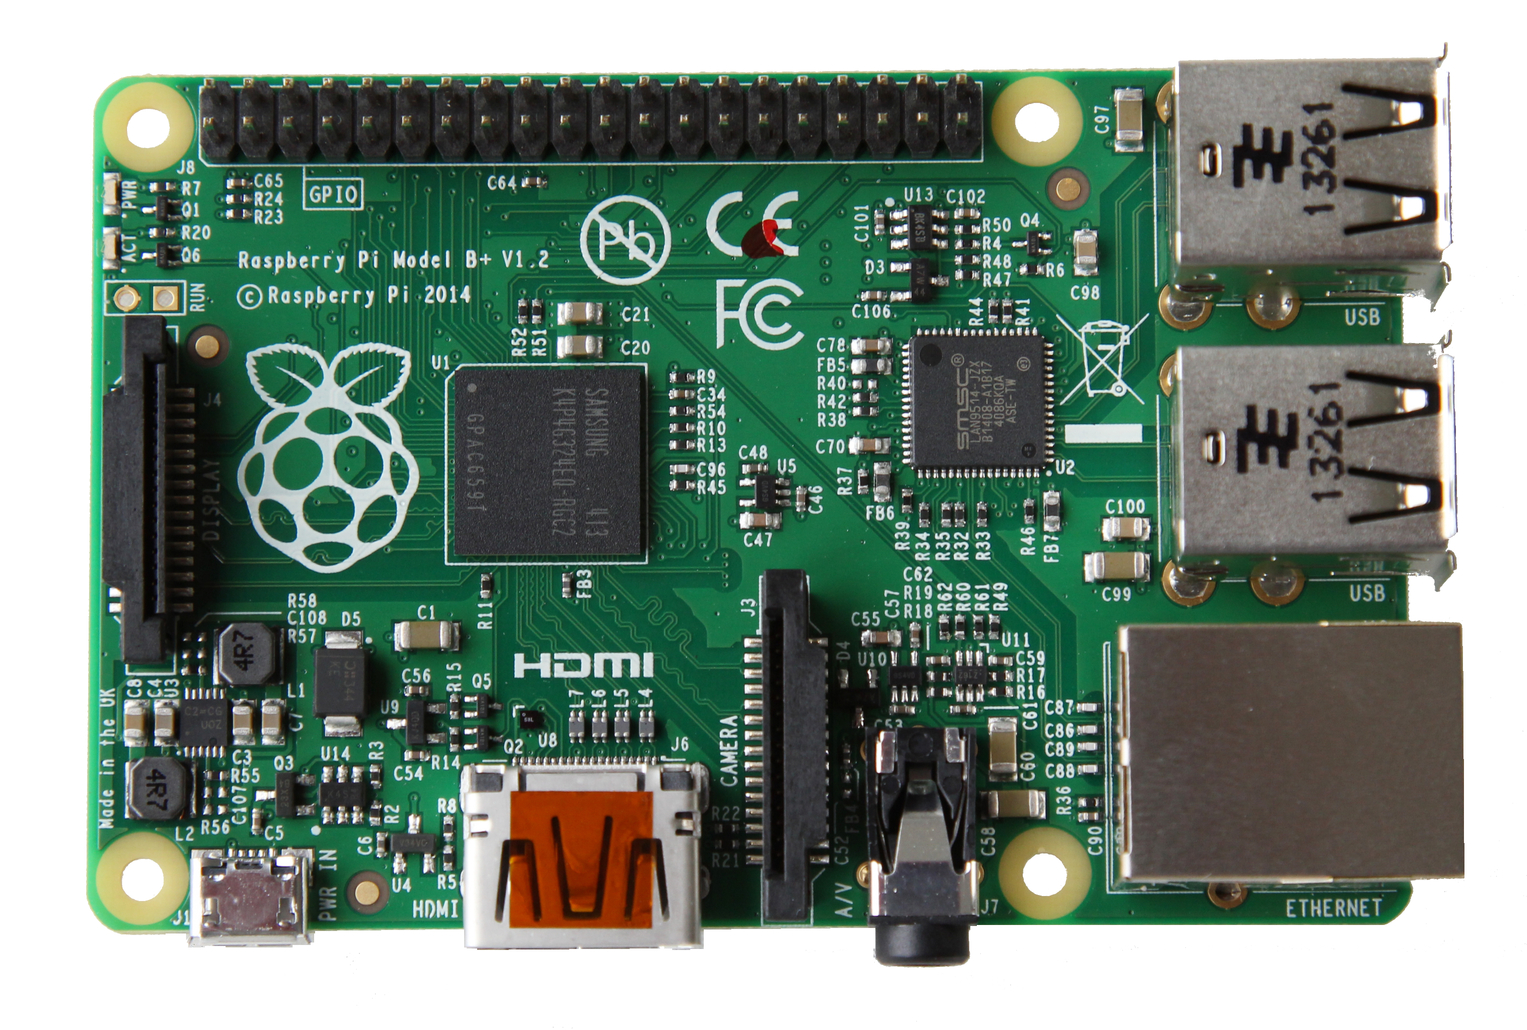
\includegraphics[width=0.5\linewidth]{img/RPi.eps}

Raspberry Pi is a single-board computer with a voltage supply of 5V (from the battery pack). The embedded operating system is Raspbian Wheezy. 
\\
The model used in the game is Raspberry Pi B+.
\\ 
Features:
\begin{enumerate}
\item 40 GPIOs (General Purpose Input/Output);
\item 4 USB ports;
\item audio output (3.5mm TRRS jack);
\item 15-pin MIPI camera interface (CSI);
\item HDMI, composite video (3.5mm TRRS jack);
\item 10/100 Mbit/s Ethernet (8P8C);
\item 512MB RAM;
\end{enumerate}
GPIOs are used to manage totem lighting and impact detection, as well as  LED lights, \textquotedblleft everything button \textquotedblright, while 2 USB ports are used for Wi-Fi network and serial communication with ARDUINO, the audio output is dedicated to sound effects. All programming was done in Python 3.
\footnote {For details on implementation, see \autoref{sec:software} and \autoref{app:code}}
It is located in the main section of the board.

\section{ARDUINO}
\label{app:Arduino}
ARDUINO is a micro controller with its own dedicated IDE and can be programmed using C++. Power supply is 5V. In the project, we used a ARDUINO UNO as a dedicated controller for managing the display in the main section of the board. 
\\
Features:
\begin{enumerate}
\item 14 digital input/output pins (of which 6 can be used as PWM outputs);
\item 6 analog inputs;
\item 16 MHz internal clock;
\item 1 USB port;
\item 1 power jack;
\item ICSP header;
\item reset button.
\end{enumerate} 

\begin{figure}
    \centering
    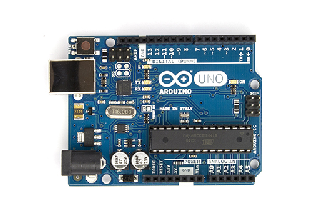
\includegraphics[width=6cm]{img/ArduinoUno}
\end{figure}

It receives serial inputs from one of the USB ports on the RPi, and uses digital outputs to control display. Inputs correspond to string of characters that should be printed on the display. The deconding of the string is left to the ARDUINO. 
It is also placed on the main section of the board.

\section{ESP}
\label{app:ESP}
ESP-12  is an ultra-low power Wi-Fi module, and can be programmed in the same way as ARDUINO. Its voltage supply is 3.3V, and offers:

\begin{figure}[h]
    \centering
    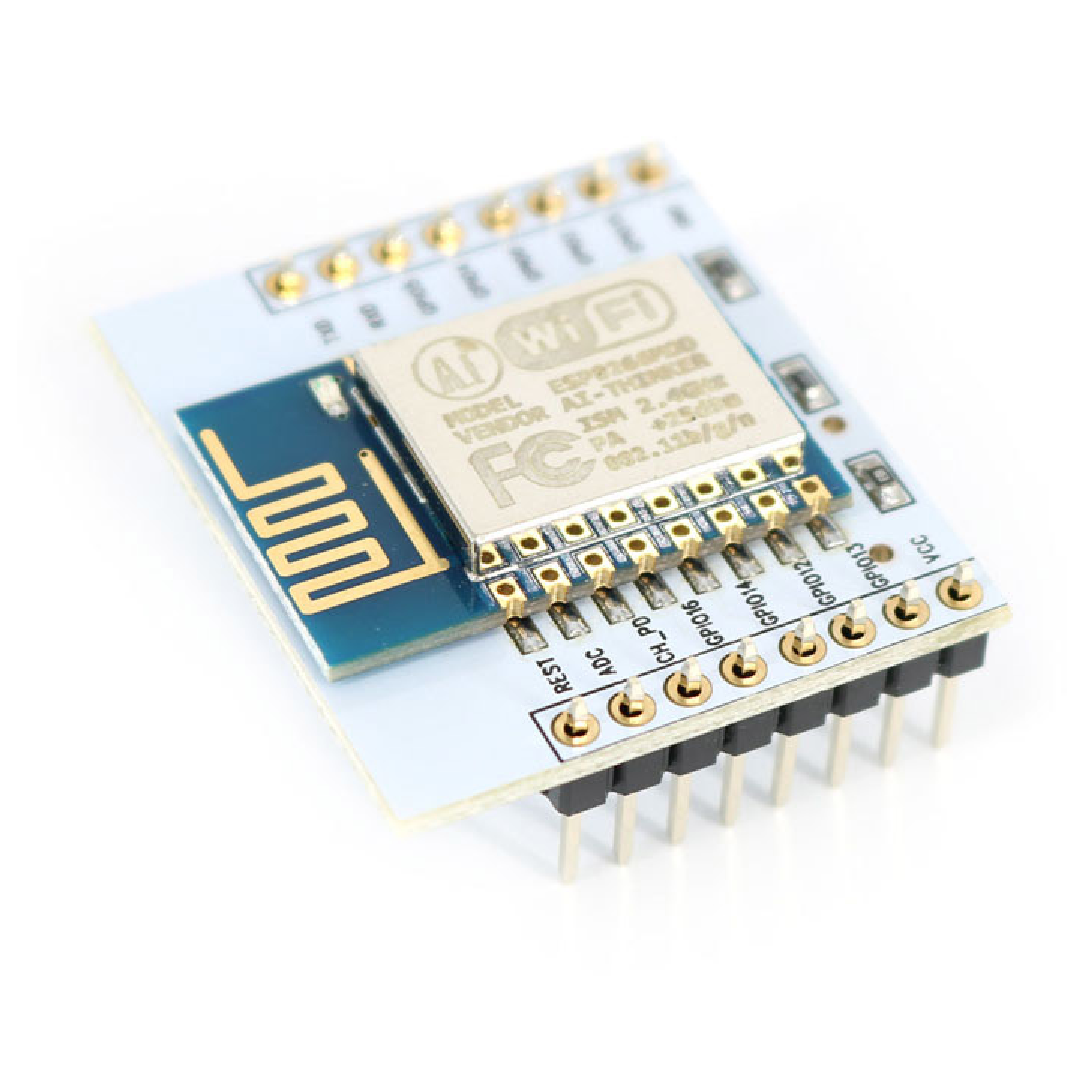
\includegraphics[width=5cm]{img/ESP12}
\end{figure}

\begin{enumerate}
\item 16 digital input/output pins (that can be used as PWM outputs);
\item Wi-Fi module;
\item ADC; 
\end{enumerate}
We chose a separate controller to use on both robot and controller, for it offered:
\begin{itemize}
\item low power consumption; 
\item smaller dimensions and reduced weight;
\item little cost (approximately 2\euro{} apiece);
\item embedded Wi-Fi (without having to use an external adapter as in Rpi).
\end{itemize}
\textbf{ESP on the controller} 
\\
The unit on the controller is responsible for:
\begin{itemize}
\item search for connection and transmitting information to the board;
\item interpretation of signals from the joystick;
\item management of LED lights.
\end{itemize}
\textbf{ESP on the robot} 
\\
The unit on the robot is responsible for:
\begin{itemize}
\item search for connection and transmitting/receiving information to and from the board;
\item driving wheels;
\item management of impact detection;
\item management of LED lights.
\end{itemize}
Because of the need to have multiple processes concurrently running, we created a scheduler to simulate parallelism on a single processor. 
\footnote {For details on implementation, see \autoref{sec:software} and \autoref{app:code}}

\section{Themes and Sounds Effects}
\label{app:noise}

All music themes come from royalty free sources:
\begin{enumerate}
\item from Creative Common Music Archives:
\begin{itemize}
\item\textquotedblleft Nachtwandel \textquotedblright, by Andy G. Cohen \textemdash  \textit{pause};
\item\textquotedblleft Rainbow Street \textquotedblright, by Scott Holmes \textemdash \textit{active play};
\item\textquotedblleft Space Outro \textquotedblright, by Andy G. Cohen \textemdash \textit{game over};
\end{itemize}
\item \textquotedblleft Acquarium\textquotedblright from \textquotedblleft Carnaval des Animaux\textquotedblright, by Camille Saint-Sa\"ens  \textemdash \textit{menu}.
\end{enumerate}
Sounds effects (such as beeps and robot squeaks) were created by us by elaborating voice recordings using Audacity. 
The format used for audio files is Ogg Vorbis, and is reproduced using VLC Media Player.

\chapter{\texttt{schemop} directives}
\label{app:schemop}
\import{app_schemop}

\chapter{FBCP commands}
\label{app:fbcp}
\import{app_fbcp}

\chapter{Code Snippets}
\label{app:code}
\import{app_code}

\end{appendices}

\bibliographystyle{plain}
\bibliography{biblio}
\end{document}

